%%%%%%%%%%%%%%%%%%%%%%%%%%%%%%%%%%%%%%%%%%%%%%%%%%%%%%%%%%%%%%%%%%%%%%
% Problem statement
\begin{statement}[
  problempoints=50,
  timelimit=1 second,
  memorylimit=512 MiB,
]{Preokret}

\setlength\intextsep{-0.1cm}
\begin{wrapfigure}[7]{r}{0.2\textwidth}
\centering
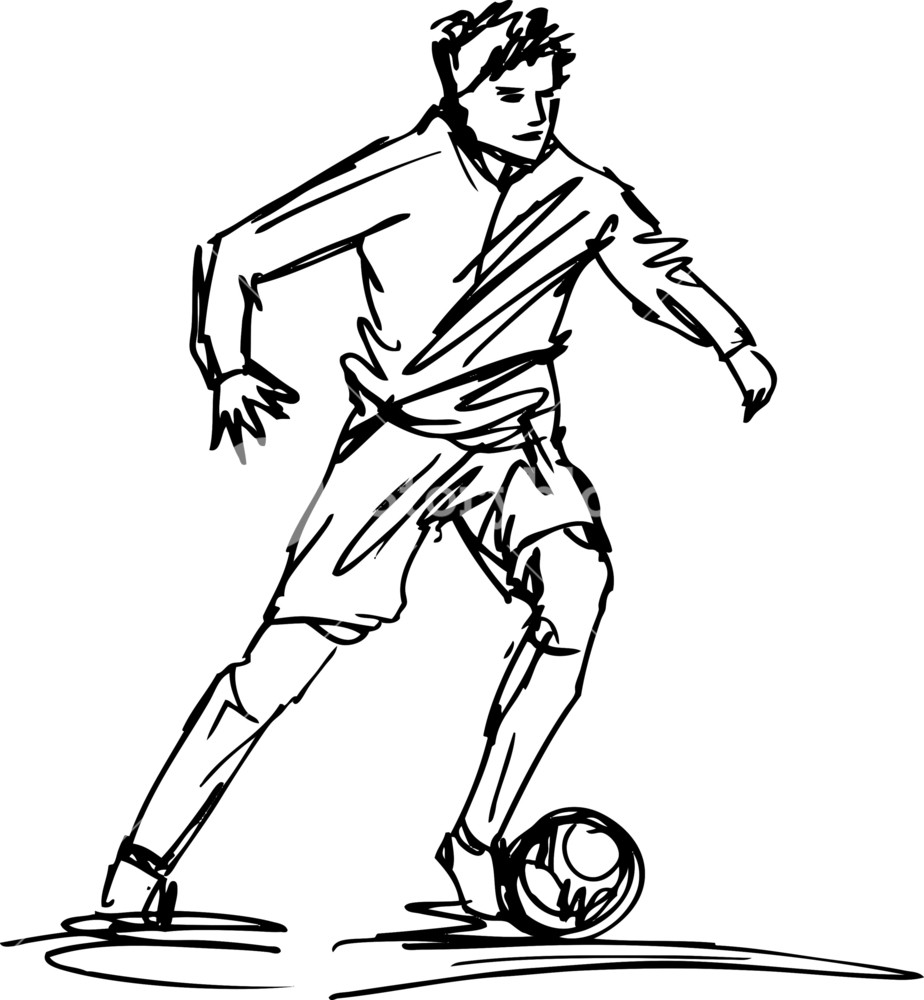
\includegraphics[width=0.2\textwidth]{img/fudbaler.jpg}
\end{wrapfigure}

It's \textit{Saint Stephen's Day}, the day after Christmas. The secular version
of the same holiday in England is known as \textit{Boxing day}. While people
in Croatia celebrate Saint Stephen's Day by stuffing themselves with
ridiculous amounts of food, our British friends traditionally play football.
Premier league, Championship, amateur leagues -- everybody plays football on
Boxing day.

This year, Pep ate too much roast beef on Christmas and decided to take a break
from Boxing day football. He stayed in bed that day, analyzing an old City
fixture against an unknown opponent.

Pep knows that there were $N$ goals scored during the match and he also knows
in which order were they scored. He watches the game and wishes to answer the
following questions

\begin{enumerate}
  \item What was the final score, i.e., how many goals did City score and how
        many goals did their opponents score?
  \item How many different ties were featured during the course of the game? We
        say that the game is tied if both teams have scored the same number of
        goals. The starting score \texttt{0:0} is also considered a tie.
  \item Let's define a \textit{turnover} as a situation in which a losing team,
        i.e. the team that scored less goals than its opponent, scores a certain
        number of successive goals and takes the lead after those goals have been
        scored. Pep wonders what is the largest turnover in the game. In other
        words, he wants to know what was the largest number of successive goals
        scored by one team such that before those goals they were losing and after
        those goals they were winning. Pep knows that this specific game had at
        least one turnover.
\end{enumerate}

%%%%%%%%%%%%%%%%%%%%%%%%%%%%%%%%%%%%%%%%%%%%%%%%%%%%%%%%%%%%%%%%%%%%%%
% Input
\subsection*{Input}
First line contains an integer $N$ $(1 \le N \le 250)$ from the task description.

In the next $N$ lines there is a single number $1$ or $2$ which represents a
team that scored a goal (in order of goals scored in the game). City is
denoted by number $1$ and their opponents by number $2$.

%%%%%%%%%%%%%%%%%%%%%%%%%%%%%%%%%%%%%%%%%%%%%%%%%%%%%%%%%%%%%%%%%%%%%%
% Output
\subsection*{Output}
In the first line you should output two space-separated integers, the number
of goals scored by City and the number of goals scored by the opposing team.

In the second line you should output the number of different ties featured
during the course of the game.

In the third line you should output the largest turnover in the game.

%%%%%%%%%%%%%%%%%%%%%%%%%%%%%%%%%%%%%%%%%%%%%%%%%%%%%%%%%%%%%%%%%%%%%%
% Scoring
\subsection*{Scoring}
In this task, each line of output is graded separately. The correct output
in the first line is worth $1$ point in each test case. The correct output
in the second line is also worth $1$ point in each test case. The correct
output in the third line is worth $3$ points in each test case.

%%%%%%%%%%%%%%%%%%%%%%%%%%%%%%%%%%%%%%%%%%%%%%%%%%%%%%%%%%%%%%%%%%%%%%
% Examples
\subsection*{Examples}
\begin{tabularx}{\textwidth}{X'X'X}
\sampleinputs{test/preokret.dummy.in.1}{test/preokret.dummy.out.1} &
\sampleinputs{test/preokret.dummy.in.2}{test/preokret.dummy.out.2} &
\sampleinputs{test/preokret.dummy.in.3}{test/preokret.dummy.out.3}
\end{tabularx}

\textbf{Explanation of the first example:}
Different scores during the game were: \texttt{0:0}, \texttt{1:0},
\texttt{2:0}, \texttt{2:1}, \texttt{2:2}, \texttt{2:3}. Out of those, there
were two ties: \texttt{0:0} and \texttt{2:2}. The largest turnover happened
when the opposing team were losing \texttt{2:0} and then scored three successive
goals, thereby winning \texttt{2:3}.

\textbf{Explanation of the second example:}
Different scores during the game were: \texttt{0:0}, \texttt{1:0},
\texttt{1:1}, \texttt{1:2}, \texttt{2:2}, \texttt{3:2}, \texttt{4:2},
\texttt{4:3}, \texttt{5:3}, \texttt{6:3}. Out of those, there were three
ties: \texttt{0:0}, \texttt{1:1} and \texttt{2:2}. The largest turnover happened
when City were losing \texttt{1:2} and then scored three successive goals and
started winning \texttt{4:2}.

%%%%%%%%%%%%%%%%%%%%%%%%%%%%%%%%%%%%%%%%%%%%%%%%%%%%%%%%%%%%%%%%%%%%%%
% We're done
\end{statement}

%%% Local Variables:
%%% mode: latex
%%% mode: flyspell
%%% ispell-local-dictionary: "croatian"
%%% TeX-master: "../hio.tex"
%%% End:
